\header{
    \headtitle{Le grand vicaire} \label{le-grand-vicaire}

    \insertComment{Publiée en 1866 sous le nom de "Curé privilégié".}{}
}

\enluminure{4}{\href{}{C}}\\ 
$\left.\begin{tabular}{l}
\hspace{-0.4cm}
\textsc{hez} nous la musique
\hspace{-0.4cm}
\\
C'est une coutume
\end{tabular}\right\rbrace$ bis
\\Mon papa fait d'l'accordéon, \bissimple
\\Ma maman fait le violon, \bissimple
\\Et le curé la viole. \bissimple
\\\textbf{Refrain :}
\\Mais le grand vicaire,
\\Toujours par derrière 
\\N'a jamais ... pu la \textit{violer},
\\Et c'est ce qui l'emmerde. \bissimple
\bisdouble{Chez nous les voyages}
{Sont fort en usage.}
\\Moi j'ai vu le Missouri, \bissimple
\\Ma femme le Mississipi, \bissimple
\\Le curé la Perse.  \bissimple
\bisdouble{Chez nous la rivière}
{Est profonde et claire.}
\\Moi je la franchie d'un bond, \bissimple
\\Ma femme la passe sur le pont, \bissimple
\\Le curé la saute. \bissimple
\bisdouble{Pour punir les gosses,}
{Je ne suis pas rosse.}
\\Je préfère les pincer, \bissimple
\\Ma femme leur fout des fessées, \bissimple
\\Le curé des calottes. \bissimple
\bisdouble{Quand un enfant se blesse,}
{Vite je m'empresse.}
\\Je cours à la pharmacie, \bissimple
\\Ma femme elle fait d'la charpie, \bissimple
\\Le curé des bandes. \bissimple
\breakpage
\bisdouble{Chez nous la coiffure}
{Fait bonne figure.}
\\Moi je porte des chapeaux melons, \bissimple
\\Ma femme des chapeaux ronds \bissimple
\\Le curé des calottes. \bissimple
\bisdouble{Chez nous, la culture}
{Est fort en usure:}
\\Moi je m'occupe de la moisson, \bissimple
\\Et ma femme de la fenaison \bissimple
\\Et le curé laboure. \bissimple
\bisdouble{Chez nous, la pendule}
{Avance et recule:}
\\Moi je m'occupe du balancier \bissimple
\\Et ma femme du boîtier, \bissimple
\\Et le curé la monte. \bissimple
\bisdouble{Chez nous les costumes}
{Sont dans la coutume;}
\\Moi, je m'occupe des pantalons \bissimple
\\Et ma femme des vestons \bissimple
\\Et le curé l'enfile. \bissimple
\bisdouble{Chez nous la charrette}
{Devant chez nous s'arrête;}
\\Moi je dételle les mulets, \bissimple
\\Ma femme défait les paquets, \bissimple
\\Et le curé décharge. \bissimple
\bisdouble{Chez nous les breuvages}
{Sont fort en usage;}
\\Moi, je prends un diabolo \bissimple
\\Et ma femme du Cointreau \bissimple
\\Et le curé la Suze. \bissimple
\bisdouble{Chez nous, la vaisselle}
{Est blanche et fort belle;}
\\Moi je récure la soupière \bissimple
\\Et ma femme la cuillère \bissimple
\\Et le curé l'astique. \bissimple
\breakpage
\bisdouble{Chez nous, le tricotage}
{Est fort en usage;}
\\Je tonds la laine des mérinos \bissimple
\\Ma femme fait des écheveaux \bissimple
\\Et le curé la pelote. \bissimple
\bisdouble{Chez nous les tentures}
{S'accrochent sur mesure;}
\\Moi, je m'occupe des anneaux \bissimple
\\Et ma femme des rideaux \bissimple
\\Et le curé de la tringle. \bissimple
\bisdouble{Chez nous, la lecture}
{Est fort en usure;}
\\Moi, je lis Victor Hugo \bissimple
\\Et ma femme Marivaux, \bissimple
\\Le curé La Condamine. \bissimple
\bisdouble{Chez nous les baskets}
{C’est une coutume}
\\Mon papa fait les Reebok, \bissimple
\\Ma maman fait Adidas, \bissimple
\\Et le curé la Nike… \bissimple
\bisdouble{Chez nous le vélo}
{C’est une coutume}
\\Mon papa fait le boyau, \bissimple
\\Ma maman fait la rustine, \bissimple
\\Et le curé la pompe… \bissimple
\bisdouble{Chez nous la basse-cour}
{C’est une coutume}
\\Mon papa fait le goret, \bissimple
\\Ma maman fait le canard, \bissimple
\\Et le curé lapine… \bissimple
\bisdouble{Chez nous les sciences}
{C’est une coutume}
\\Mon papa fait la physique, \bissimple
\\Ma maman fait la bio, \bissimple
\\Et le curé les maths… \bissimple
\breakpage
\bisdouble{Chez nous la géo}
{C’est une coutume}
\\Mon papa fait la boussole, \bissimple
\\Ma maman fait le compas, \bissimple
\\Et le curé l’écarte… \bissimple
\bisdouble{Chez nous la maçonnerie}
{C’est une coutume}
\\Mon papa fait le mortier, \bissimple
\\Ma maman fait la truelle, \bissimple
\\Et le curé l’embrique… \bissimple
\bisdouble{Chez nous la gymnastique}
{C’est une coutume}
\\Mon papa fait le salto, \bissimple
\\Ma maman fait la rondade, \bissimple
\\Le curé la culbute… \bissimple
\bisdouble{Chez nous les voyages}
{C’est une coutume}
\\Mon papa il fait l’Egypte, \bissimple
\\Ma maman la Macédoine, \bissimple
\\Et le curé la Perse… \bissimple
\bisdouble{Chez nous être malade}
{C’est une coutume}
\\Mon papa a la gastro \bissimple
\\Ma maman elle fait la grippe, \bissimple
\\Et le curé la crève… \bissimple
\bisdouble{Chez nous l’anatomie}
{C’est une coutume}
\\Mon papa il fait les jambes, \bissimple
\\Ma maman elle fait les bras, \bissimple
\\Et le curé la tronche… \bissimple
\bisdouble{Chez nous le football}
{C’est une coutume}
\\Mon papa tire les pénaux, \bissimple
\\Ma maman fait les corners, \bissimple
\\Et le curé la touche… \bissimple
\breakpage
\bisdouble{Chez nous la vaisselle}
{C’est une coutume}
\\Mon papa c’est Paic citron, \bissimple
\\Ma maman c’est le torchon, \bissimple
\\Et le curé l’éponge… \bissimple
\bisdouble{Chez nous les bébés}
{C’est une coutume}
\\Mon papa c’est le biberon, \bissimple
\\Ma maman c’est la tétine, \bissimple
\\Et le curé la couche… \bissimple
\bisdouble{Chez nous Star Wars}
{C’est une coutume}
\\Mon papa se tape Léia, \bissimple
\\Ma maman c’est Chewbacca, \bissimple
\\Et le curé la Force… \bissimple
\bigskip
\begin{center}
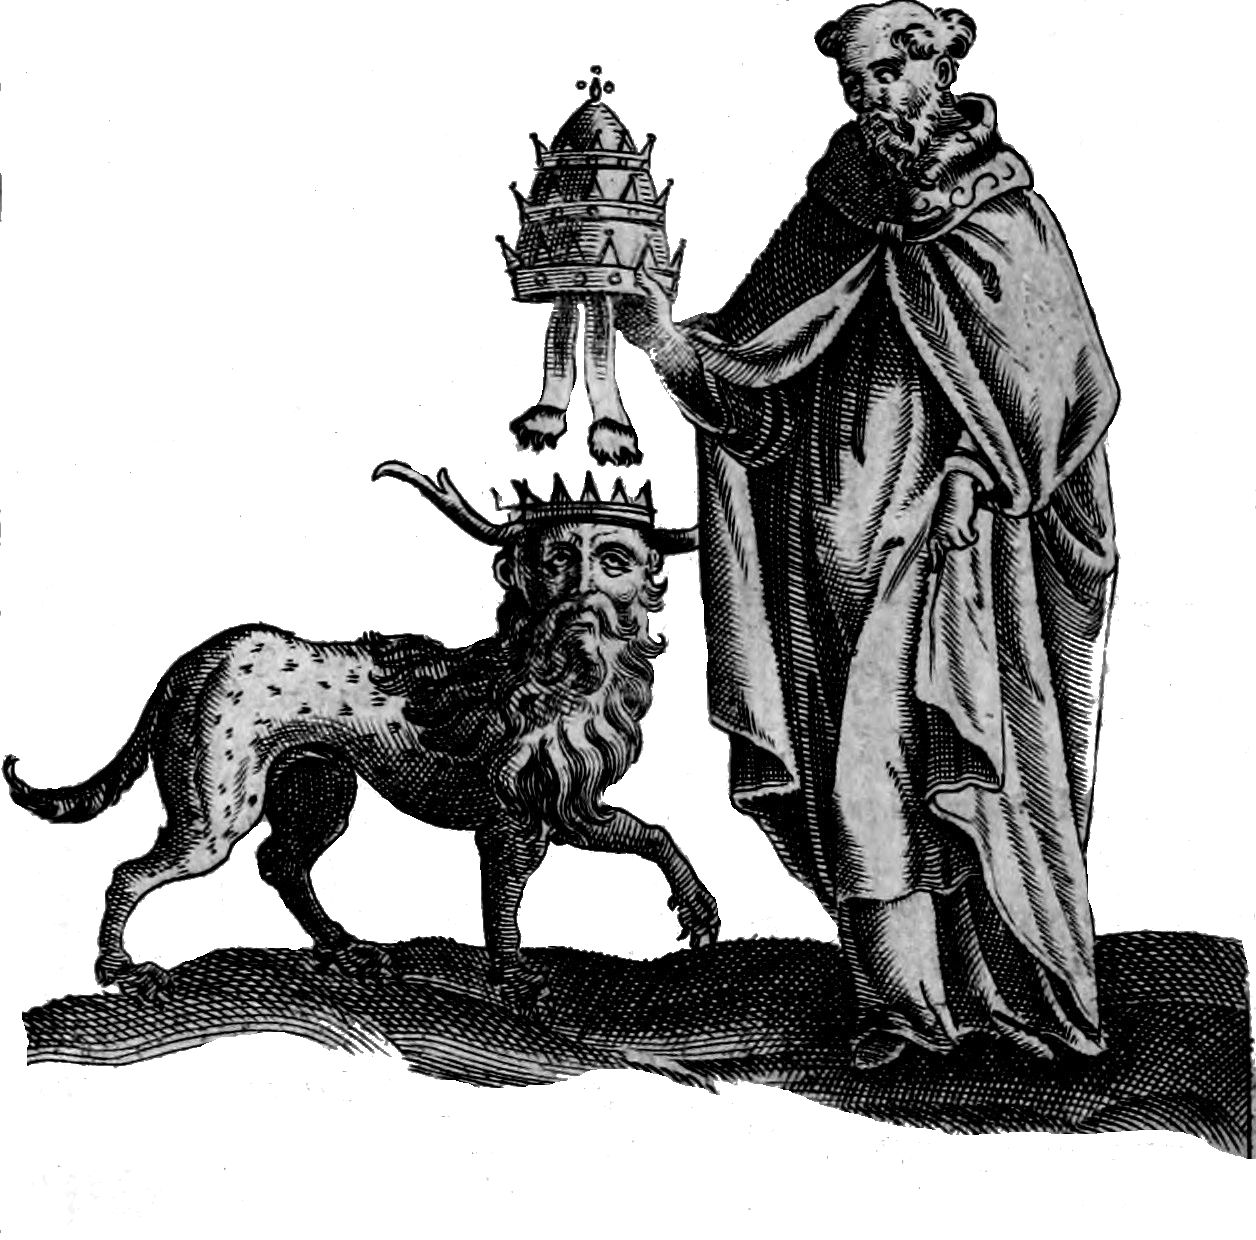
\includegraphics[width=0.9\textwidth]{images/brev38.png}
\end{center}

\breakpage